\epi{"There and back again."}{Bilbo Baggins}
\noindent{}There are a few things that make Go different than most other language
out there.
\begin{description}
\item[Clean and Simple]
Go strives to keep things small and beautifull, you should
be able to do impressive things in a few lines of code;
\item[Concurrent]
Go makes it easy to ''fire off'' functions to be
run as \emph{very} lightweight threads. These threads are called
\first{go-routines} in Go;

\item[Channels] 
Communication with these go-routines is done
via \first{channels} \cite{csp}\cite{ohoare};

\item[Fast]
Compilation is fast and execution as fast. The aim is
to be as fast as C. Compilation time is measured in seconds;

\item[Safe]
Go has garbage collection, no more \func{free()} in Go,
the language takes care of this;

\item[Standard format]
A Go program can be formatted in (almost) any way the programmmers want,
\emph{but} an official format exist. The rule is very simple:
The output of the filter \prog{gofmt} \emph{is} the official endorsed
format.

\item[Postfix types]
Types are given \emph{after} the variable name, thus \prog{var a int},
instead of \prog{int a;} as in C;

\item[UTF-8]
UTF-8 is all over the place, in strings
\emph{and} in the program code. Finally you can use \prog{$\Phi$ =
$\Phi$ + 1} in your source code;

\item[Open Source]
The Go license is completely open source, see the file LICENSE in the Go
source code distribution;

\item[Fun]
Programming with Go should be fun again!

\end{description}
It must be said the Erlang \cite{erlang} and Scala \cite{scala} also share some
of the features of Go. Notible differences between Erlang
and Go is that Erlang borders on being a functional language,
where Go is an imperative one. And Erlang is running a virtual
machine, while Go is compiled. 

Scala runs on the JVM (Java Virtual Machine) and is thus compiled 
bytecode. Is shares features with both Go and Erlang, but still\ldots
JVM.  Well, on with Go.

\section{Hello World}
\label{sec:hello world}
In the Go tutorial, Go is presented to the world in the typical
manner: letting it print "Hello World" (Heck! Ken Thompson and
Dennis Ritchie started this when they presented the C language in 
the nineteen seventies).
So here it is, ''Hello World'' in Go.

\lstinputlisting[numbers=right,label=src:hello,caption=Hello world]{src/helloworld.go}
As you can see, Go is 100\% UTF-8 capable, you can put any Unicode
glyph in your source - assuming you can type it on your keyboard.
Go supports both the \texttt{\rem{/* */}} and \texttt{\rem{//}} types of comments. 

Line 1 is just required.  All Go files start with \lstinline{package <something>}.
\lstinline{package main} is required for a standalone executable.  Line 3 says
we need \package{"fmt"} in addition to \package{main}.  A package other than
main is commonly called a library, a familiar concept of many programming
languages (See chapter \ref{chap:packages}. 
Just as \lstinline{package main} was required to be first, 
\lstinline{import} must come next. Always in Go, package is first, then import, 
then everything else.

\section{Compiling and running code}
This is a very concise instruction on how to get your code
compiled and get it running.
The shortest program you can write in Go looks like
this:
%%\lstinputlisting[numbers=right,label=src:short,caption=Shortest Go program]{src/short.go}
In which we define the \key{package} \package{main} and supply it with one
function also called \func{main()}. The fully qualified function
name is \func{main.main()}. Go always calls \func{main.main()} automatically.

To compile we do the following

\begin{display}
\pr 8g helloworld.go \qquad\qquad\qquad\rem{# compiles to helloworld.8 (for 32 bit Intel)}
\pr 8l -o helloworld helloworld.8 \qquad\rem{# linking stage}
\end{display}
For 64 bit Intel you should use \prog{6g} and \prog{6l}, this will
generate \prog{helloworld.6}.

After getting this compiled we can run it:
\begin{display}
\pr ./helloworld
\end{display}\texttt{Hello, world; or }%
\begin{math}\kappa\alpha\lambda\eta\mu\acute{\epsilon}\rho\alpha\hspace{1em}\kappa\end{math}%
\'o\begin{math} \sigma\mu\epsilon\end{math}; or \begin{cjk}こんにちは 世界\end{cjk}
\ \newline
\ \newline
In the next sections we will look at the types, keywords, control structures
and other features of our new language. 

\section{Variables, types and keywords}
Go is different than other languages in that the type of a variable
is specified \emph{after} the variable name. So no: 
\lstinline{int a}, but \lstinline{a int}. When declaring a variable it
is assigned the "natural" zero value for the type. This means that after
\lstinline{var a int}, \lstinline{a} has the value $0$. With
\lstinline{var s string}, \lstinline{s} is assigned the zero string,
which is \lstinline{""}.

\subsection{Nil value}
A reference to nothing is represented in Go as \lstinline{nil}. This is
different than a zero value. \draft{nil only for references?}

\begin{lstlisting}
var *a int
a = nil
fmt.Printf("%v\n", a);
\end{lstlisting}
Prints \lstinline{nil}.

\subsection{Boolean types}
A boolean type represents the set of Boolean truth values denoted by the
predeclared constants \emph{true} and \emph{false}. The predeclared boolean type is \type{bool}.

\subsection{Numerical types}
Go has the well known types such as \lstinline{int} and
\lstinline{float}. These types have the appropriate length for your
machine. If you want to be explicit about the length you can have
that too with \lstinline{int32}, or \lstinline{uint32}. Note however
that these types are distinct and assigning variables which mix
these types is a compiler error. Like in the following code:

\lstinputlisting[numbers=right,label=src:types,caption=Familiar types are still distinct]{src/types.go}
Gives the error on the assignment on line 7:

\noindent\lstinline{types.go:7: cannot use a + a (type int) as type int32 in assignment}

\subsection{Strings}
An important other built in type is \lstinline{string}. Strings in Go are
immutable, meaning that, once defined, they can not be changed. For
people coming from C, the following is not legal in Go:
\lstinline{var s string = "hello"; s[0] = 'c'} 
In Go you will need the following:
\begin{lstlisting}
s := "hello"
c := []int(s)	    |\longremark{Convert \texttt{s} to an array;}|
c[0] = 'c'	    |\longremark{Change the first element of this %
array;}|
s2 := string(c[0]) + string(c[1:]) |\longremark{Create a \emph{new} %
string \texttt{s2} with the alteration.}|
fmt.Printf("%v\n", s2)
\end{lstlisting}

\showremarks

\subsection{Constants}
iota, and more about constants\draft{TODO}

\subsection{Complex numbers}
\gomarginpar{Complex numbers were added on 18 February 2010. \hg{2010-02-18}}
In Go we have native support for complex numbers. If you 
want use them you need a variable of the type \lstinline{complex}. If
you need a precise number of bits you have \lstinline{complex32} and
\lstinline{complex64} for 32 and 64 bits. A small example of using complex numbers:

\lstinline{var c complex = 5+5i; fmt.Printf("Value is: %v", c")}, will
print \lstinline{(5+5i)}.

\subsection{Go keywords}
\begin{table}[H]
\begin{center}
\caption{Keywords in Go}
\label{tab:keywords}
%%%%%%%%%%%%%%%%%%%%%%%%%%%%%%%%%%%%%%%%%%%%%%%%%%%%%%%%%%%%%%%%%%%%%%
%%                                                                  %%
%%  This is a LaTeX2e table fragment exported from Gnumeric.        %%
%%                                                                  %%
%%%%%%%%%%%%%%%%%%%%%%%%%%%%%%%%%%%%%%%%%%%%%%%%%%%%%%%%%%%%%%%%%%%%%%
\begin{tabular}{lllll}
\key{break}	&\key{default}          &\key{for}	&\key{import}    &\key{return}\\
\key{case}	&\key{defer}            &\key{func}	&\key{interface}          &\key{select}\\
\key{chan}	&\key{delete}           &\key{go}	&\key{map}      &\key{struct}\\
\key{const}	&\key{else}    	    &\key{goto}	&\key{package}        &\key{switch}\\
\key{continue}	&\key{fallthrough}      &\key{if}	&\key{range}       &\key{type}\\
               &                       &               &                   &\key{var}\\
\end{tabular}

\end{center}
\end{table}
Table \ref{tab:keywords} lists all the keywords in Go.
In the following paragraphs and chapters we will explain some of
them. \draft{TODO make references from here to chapters where they are
explained.}

\section{Built-in functions}
A number of functions in Go are predefined, meaning they already
\gomarginpar{This is list changing (slowly).\hg{2010-02-04}}
exists and you \emph{don't} have to include any package to get
access to them. In the following paragraphs we list the current 
built-in functions. This is copied from \cite{go_spec}.

\paragraph{\func{close} and \func{closes}} are used in
channel closing (see chapter \ref{chap:channels}).

\paragraph{\func{len} and \func{cap}} are the length and the capacity
of a \type{slice} or an \type{array} respectively. Also see
\ref{capacity}.

\paragraph{\func{new}} is used for creating new ... See allocation. CODE
EXMAPLES

\paragraph{\func{make}} is used for allocating a built-in type. EXAMPLE
TODO

\paragraph{\func{copy}} copy stuff. TODO

\paragraph{\func{panic} and \func{panicln}} used for an elegant \emph{exception} mechanism.
CODE EXAMPLES

\paragraph{\func{print} and \func{println}} are lowlevel printing
functions that can be used without reverting to the \package{fmt} package.

\paragraph{\func{cmplx}, \func{real} and \func{imag}} all deal with
complex numbers.

\section{Control structures}
The control structures of Go are related to those of C but different in
\gomarginpar{This section is from \cite{effective_go}.}
important ways. There is no do or while loop, only a slightly
generalized \key{for}; \key{switch} is more flexible; \key{if} and
\key{switch} accept an
optional initialization statement like that of \key{for}; and there are new
control structures including a type switch and a multiway communications
multiplexer, \key{select}. The syntax is also slightly different: parentheses
are not required and the bodies must \emph{always} be brace-delimited.

\subsection{If}
In Go a simple if looks like this:
\begin{lstlisting}
if x > 0 {
    return y
}
\end{lstlisting}
Mandatory braces encourage writing simple \key{if} statements on multiple
lines. It's good style to do so anyway, especially when the body
contains a control statement such as a \key{return} or \key{break}.

Since \key{if} and \key{switch} accept an initialization statement, it's common to
see one used to set up a (local) variable.

\begin{lstlisting}
if err := file.Chmod(0664); err != nil {
    log.Stderr(err)
    return err
}
\end{lstlisting}
In the Go libraries, you'll find that when an \key{if} statement doesn't flow
into the next statement-that is, the body ends in \key{break},
\key{continue}, \key{goto},
or \key{return}, the unnecessary \key{else} is omitted.

\begin{lstlisting}
f, err := os.Open(name, os.O_RDONLY, 0)
if err != nil {
    return err
}
codeUsing(f)
\end{lstlisting}
This is a example of a common situation where code must analyze a
sequence of error possibilities. The code reads well if the successful
flow of control runs down the page, eliminating error cases as they
arise. Since error cases tend to end in \key{return} statements, the resulting
code needs no \key{else} statements.
\begin{lstlisting}
f, err := os.Open(name, os.O_RDONLY, 0)
if err != nil {
    return err
}
d, err := f.Stat()
if err != nil {
    return err
}
codeUsing(f, d)
\end{lstlisting}

\subsection{For}
The Go \key{for} loop is similar to-but not the same as-C's. It unifies for
and while and there is no do-while. There are three forms, only one of
which has semicolons.
\begin{lstlisting}
// Like a C for
for init; condition; post { }

// Like a C while
for condition { }

// Like a C for(;;)
for { }
\end{lstlisting}
Short declarations make it easy to declare the index variable right in the loop.
\begin{lstlisting}
sum := 0
for i := 0; i < 10; i++ {
    sum += i
}
\end{lstlisting}
If you're looping over an array, slice, string, or map, or reading from
a channel, a \key{range} clause can manage the loop for you.
\begin{lstlisting}
var m map[string]int
sum := 0
for _, value := range m {  // key is unused
    sum += value
}
\end{lstlisting}
For strings, the \key{range} does more work for you, breaking out individual
Unicode characters by parsing the UTF-8 (erroneous encodings consume one
byte and produce the replacement rune U+FFFD). The loop

\begin{lstlisting}
for pos, char := range "a|$\Phi{}$|x" {
    fmt.Printf("character \'%c\' starts at byte position %d\n", char, pos)
}
\end{lstlisting}
prints
\begin{display}
character a starts at byte position 0
character \begin{math}\Phi\end{math} starts at byte position 1
character x starts at byte position 3
\end{display}
Finally, since Go has no comma operator and ++ and \-\- are statements not
expressions, if you want to run multiple variables in a \key{for} you should
use parallel assignment.
\begin{lstlisting}
// Reverse a
for i, j := 0, len(a)-1; i < j; i, j = i+1, j-1 {
    a[i], a[j] = a[j], a[i]
}
\end{lstlisting}

\subsection{Switch}
Go's \key{switch} is more general than C's. The expressions need not be
constants or even integers, the cases are evaluated top to bottom until
a match is found, and if the \key{switch} has no expression it switches on
\type{true}. It's therefore possible - and idiomatic - to write an
\key{if-else-if-else}
chain as a \key{switch}.
\begin{lstlisting}
func unhex(c byte) byte {
    switch {
    case '0' <= c && c <= '9':
        return c - '0'
    case 'a' <= c && c <= 'f':
        return c - 'a' + 10
    case 'A' <= c && c <= 'F':
        return c - 'A' + 10
    }
    return 0
}
\end{lstlisting}
There is no automatic fall through, but cases can be presented in comma-separated lists.

\begin{lstlisting}
func shouldEscape(c byte) bool {
    switch c {
    case ' ', '?', '&', '=', '#', '+', '%':
        return true
    }
    return false
}
\end{lstlisting}
Here's a comparison routine for byte arrays that uses two \key{switch} statements:

\begin{lstlisting}
// Compare returns an integer comparing the two byte arrays
// lexicographically.
// The result will be 0 if a == b, -1 if a < b, and +1 if a > b
func Compare(a, b []byte) int {
    for i := 0; i < len(a) && i < len(b); i++ {
        switch {
        case a[i] > b[i]:
            return 1
        case a[i] < b[i]:
            return -1
        }
    }
    switch {
    case len(a) < len(b):
        return -1
    case len(a) > len(b):
        return 1
    }
    return 0
}
\end{lstlisting}
A switch can also be used to discover the dynamic type of an interface
variable. Such a type switch\gomarginindex{\emph{type switch}}{type switch} uses 
the syntax of a type assertion with the keyword type inside the
parentheses. If the switch declares a variable in the expression, the
variable will have the corresponding type in each clause.

\begin{lstlisting}
switch t := interfaceValue.(type) { |\coderemark{Yes, you need to type \texttt{(type)}}|
default:
    fmt.Printf("unexpected type %T", t)  // %T prints type
case bool:
    fmt.Printf("boolean %t\n", t)
case int:
    fmt.Printf("integer %d\n", t)
case *bool:
    fmt.Printf("pointer to boolean %t\n", *t)
case *int:
    fmt.Printf("pointer to integer %d\n", *t)
}
\end{lstlisting}

\section{Arrays, slices and maps}
From \cite{go_intro} ... really Good
%
arrays, even if it doesn't have any other parametric types? And we really want
these cool things called slices - but they really need to be strongly typed. So
we'll let them be parametric. And maps - we really need a map type, which maps
keys to values, and it really needs to be type-safe. So we'll add a parametric
map type to the language, by making it a special case built-in.

So: you can't write parametric types - but they can. And that creates a very
weird asymmetry to the language. Everything in Go is passed by value - except
for the built-in slice and map types, which are passed by reference. Everything
is allocated by "new" - except for the built-in slice and map types, which are
allocated by "make". It's by far the biggest blemish in Go, and it's absolutely
infuriating.

\subsection{Arrays}
Array types like \lstinline{[10]int} have a fixed size. 
It can't grow, because then it would have a different type. Also arrays
are values: Assigning one array to another \emph{copies} all the elements.

In particular, if you pass an array to a function, it will receive a
copy of the array, not a pointer to it. This is a major difference with C.

To declare an array you can use the following: \lstinline{var a [3]int},
to initialize it to something else than zero, use a composite literal.
\gomarginindex{composite literals}{composite literals}\lstinline|a := [3]int{1, 2, 3}| and
this can be shortend to \lstinline|a := []int{1, 2, 3}|, where Go counts
the elements automatically.

Note that all fields must be specified.  So if you are using multidimentional
arrays you have to do quite some typing:
\begin{lstlisting}
a := [2][2]int{ [2]int{1,2}, [2]int{3,4} }
\end{lstlisting}
Which is \emph{not} the same as:
\begin{lstlisting}
a := [2][2]int{ []int{1,2}, []int{3,4} }
\end{lstlisting}
As this gives a compile error.\draft{why?}\newline
\lstinline{cannot use slice literal (type []int) as type [2]int in array index}

But this is then OK again:
\begin{lstlisting}
a := [][]int{ []int{1,2}, []int{3,4} }
\end{lstlisting}  
So either specify the length of the array or let Go do the counting, but
don't mix the two.

\subsection{Slices}
Slices are reference types, which means that if you assign one slice to
another, both refer to the same underlying array. For instance, if a
function takes a slice argument, changes it makes to the elements of the
slice will be visible to the caller, analogous to passing a pointer to
the underlying array. A slice is always coupled to an array that has
a fixed size. For slices we define a capacity and a length.

\begin{figure}[!bh]
\caption{Array versus slice}
\label{fig:array-vs-slice}
\begin{center}
\includegraphics[scale=0.65]{fig/array-vs-slice.pdf}
\end{center}
\end{figure}
Figure \ref{fig:array-vs-slice} depicts the following Go code.
First we create an array of $m$ elements of the type \lstinline{int}:
\lstinline{var array[m + 1]int}\newline
Next, we create a slice from this array: 
\lstinline{slice := array[0:n +1]}\newline
And now we have:
\begin{itemize}
\item{\lstinline{len(slice) = n, cap(slice) = m};}
\item{\lstinline{len(array) = cap(array) = m}.}
\end{itemize}
Also see the following code:
\lstinputlisting[numbers=right,label=src:arrays,caption=Arrays and slices]{src/array-and-slices.go}
On line 8 we dare to do to impossible and try to allocate something
behind the capacity (maximum length of the under laying array) and
we are greeted with a \emph{runtime} error 

\noindent\lstinline{throw: index out of range}.

\subsection{Maps}
\label{sec:maps}

\section{Conversions}
\label{sec:conversions}
Sometimes you want to convert a type to another type. In C this is known
as casting a value to another type. This is also possible in Go, but
there are some rules.\draft{there are more rules, but we're trying to
keep it simple...}
You can convert:
\begin{itemize}
\item{
From a \lstinline{string} to a slice of \lstinline{byte}s.
\begin{lstlisting}
mystring = "hello this is string"
byteslice =  []byte(mystring)
\end{lstlisting}
}
\item{
From a slice of \lstinline{byte}s to a \lstinline{string}.
\begin{lstlisting}
The other way around
\end{lstlisting}
}
\end{itemize}
\draft{Maybe put this to the end of this chapter}
%%x is an integer or has type []byte or []int and T is a string type.
%%and back
%% integer/float truncation



\section{Exercises}
\begin{Exercise}[title={For-loop},difficulty=1]
\label{ex:for-loop}
\Question \label{ex:for-loop q1} Create a simple loop with the \key{for} construct. Make it loop
10 times and print out the loop counter with the \package{fmt} package.

\Question \label{ex:for-loop q2} Rewrite the loop from 1. to use \key{goto}. The
keyword \key{for} may not be used.

\Question \label{ex:for-loop q3} Write the loop so that it fills and array and in
another loop prints it to the screen.
\end{Exercise}

\begin{Answer}

\Question There are a multitude of possibilities, 
one of the solutions could be:
\lstinputlisting[label=src:for,caption=Simple for-loop]{ex-basics/src/for.go}
Lets compile this and look at the output.
\vskip\baselineskip
\begin{display}
\pr 6g for.go && 6l -o for for.8
\pr ./for
0
1
.
.
.
9
\end{display}
\vskip\baselineskip

\Question Rewriting the loop results in code that should look something
like this (only showing the \func{main}-function):
\begin{lstlisting}
func main() {
        i := 0		|\coderemark{Define our loop variable}|
I:			|\coderemark{Define a label}|
        fmt.Printf("%d\n", i)
        i++ 
        if i < 10 {
                goto I	|\coderemark{Jump back to the label}|
        }   
}
\end{lstlisting}

\Question TODO.
\end{Answer}


\begin{Exercise}[title={字符串},difficulty=1]
\label{ex:strings}
\Question \label{ex:strings q1} 建立一个~Go 程序打印下面的内容(到~100 个字符):
\vskip\baselineskip
\begin{display}
A
AA
AAA
AAAA
AAAAA
AAAAAA
AAAAAAA
...
\end{display}
\vskip\baselineskip

\Question \label{ex:strings q2} 建立一个程序统计字符串里的字符数量:
\begin{display}
asSASA ddd dsjkdsjs dk
\end{display}
同时输出这个字符串的字节数。
\emph{提示:} 看看~\package{unicode/utf8} 包。

\Question \label{ex:string q3} 扩展上一个问题的程序,替换位置~4 开始的三个字符为~``abc''。

\Question \label{ex:string q4} 编写一个~Go 程序可以逆转字符串,例如``foobar''
被打印成``raboof''。
\emph{提示:}不幸的是你需要知道一些关于转换的内容,
参阅``\titleref{sec:conversions}''第~\pageref{sec:conversions} 页的内容。

\end{Exercise}

\begin{Answer}

\Question 这是一个解法:

\lstinputlisting[label=string1,caption=字符串]{ex-basics/src/string1.go}

\Question 为了解决这个问题,需要~\package{unicode/utf8} 包的帮助。
首先,阅读一下文档~\prog{go doc unicode/utf8 | less}。在阅读文档的时候,会注意到
\lstinline{func RuneCount(p []byte) int}。然后,将~
\emph{string} 转换为~\type{byte} slice:
\begin{lstlisting}
str := "hello"
b   := []byte(str) |\coderemark{转换,参阅第~\pageref{sec:conversions} 页}|
\end{lstlisting}

将这些整合到一起,得到下面的程序。

\begin{minipage}{\textwidth}
\lstinputlisting[label=src:string2,caption=字符串中的 rune]{ex-basics/src/string2.go}
\end{minipage}
\Question 将此作为练习留给读者。如果你完成了它,请同我联系!
我将会把你的答案放在这里。

\Question 可以用下面的方法逆转字符串。我们从左边(\var{i})至右(\var{j})的交换字符,就像这样:

\begin{minipage}{\textwidth}
\lstinputlisting[label=src:stringrev,caption=逆转字符串,linerange={3,}]{ex-basics/src/stringrev.go}
\end{minipage}

\end{Answer}


\cleardoublepage
\section{Answers}
\shipoutAnswer
